\documentclass[uplatex,a4paper,dvipdfmx,titlepage,oneside,openany]{jsarticle}

\usepackage{amsmath,amsthm,amsfonts,latexsym,mathtools,bm,ulem,amssymb,tikz,circuitikz,graphicx}

\usepackage{times}
\usepackage[subrefformat=parens]{subcaption}
\usepackage{here}
\usepackage{siunitx}
\usepackage{physics}
\usepackage{upgreek}%ギリシャ文字を立てる
\usepackage{tikz-3dplot}
\begin{document}
	\begin{figure}[H]
		\centering
		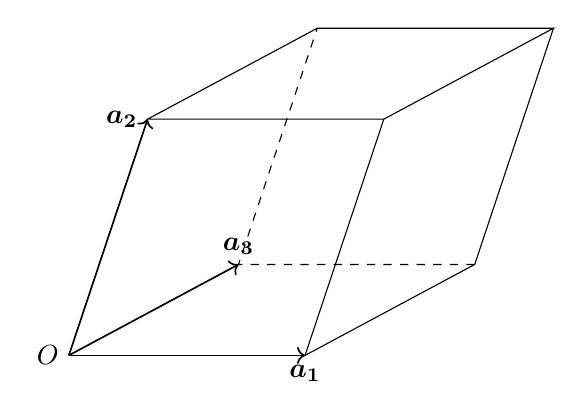
\begin{tikzpicture}
			\draw[->,semithick] (0,0,0) node[left]{$O$}--++(3,0,0) node[below]{$\bm{a_1}$};
			\draw[->,semithick] (0,0,0)--++(1,3,0) node[left]{$\bm{a_2}$};
			\draw[->,semithick] (0,0,0)--++(1,0,-3) node[above]{$\bm{a_3}$};
			\draw[] (3,0,0) --++(1,3,0)--++(-3,0,0)--++(1,0,-3)--++(3,0,0)--++(-1,0,3);
			\draw[] (3,0,0) --++(1,0,-3)--++(1,3,0);
			\draw[dashed] (4,0,-3)--++(-3,0,0)--++(1,3,0);
		\end{tikzpicture}
	\end{figure}
		\tdplotsetmaincoords{0}{-20}
		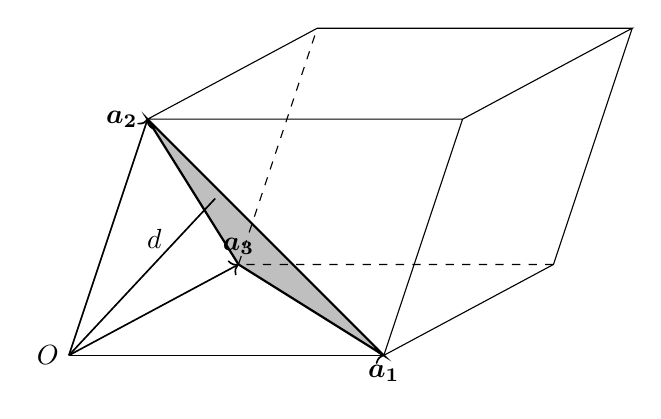
\begin{tikzpicture}
			\draw[thick,fill=lightgray] (4,0,0)--++(-3,3,0)--++(0,-3,-3)--++(3,0,3)--cycle;
			\draw[->,semithick] (0,0,0) node[left]{$O$}--++(4,0,0) node[below]{$\bm{a_1}$};
			\draw[->,semithick] (0,0,0)--++(1,3,0) node[left]{$\bm{a_2}$};
			\draw[->,semithick] (0,0,0)--++(1,0,-3) node[above]{$\bm{a_3}$};
			\draw[semithick,-.] (0,0,0)--++(1+0.5,4/3+0.3,-4/3+0.4);
			\node at(0.7,1.1,-1){$d$};
			\draw[] (4,0,0) --++(1,3,0)--++(-4,0,0)--++(1,0,-3)--++(4,0,0)--++(-1,0,3);
			\draw[] (4,0,0) --++(1,0,-3)--++(1,3,0);
			\draw[dashed] (5,0,-3)--++(-4,0,0)--++(1,3,0);
		\end{tikzpicture}
\end{document}